\documentclass{article}

\usepackage[english]{babel} %Forces American English hyphenation patters
\usepackage[utf8x]{inputenc} % Unicode
\usepackage{amsmath, amssymb, amsthm} %AMS Math Packages
\usepackage{textcomp, siunitx, gensymb, wasysym} %Symbol Packages, Textcomp removes certain errors
\usepackage{multicol, geometry, fancyhdr,indentfirst} %Page Layout Packages 
\usepackage{graphicx, wrapfig, subcaption} %Figure Packges



\newcommand{\e}[1]{\times 10^{#1}}
\newcommand{\Lim}[1]{\underset{#1}{\lim}}
\newcommand{\abs}[1]{\lvert #1 \rvert}
\newcommand{\norm}[1]{\lVert #1 \rVert}
\newcommand{\Rom}[1]{\MakeUppercase{\romannumeral #1}}
\newcommand{\rom}[1]{\romannumeral #1}
\renewcommand{\l}{\left}
\renewcommand{\r}{\right}

\pagestyle{fancyplain}
\headheight 1cm
\lhead{Michael Dymek \\ \today}
\chead{\textbf{\Large Final Project}}
\rhead{Dr. Amy Anderson \\ Math 342}
\headsep .5cm


\begin{document}
\section*{Abstract}
	I will be using WHO data to analyze the affect of 13 different predictor variables on the life expectancy of a given country in the year 2015. With this dataset, I will be asnwering the following questions.
	\begin{enumerate}
		\item Do the various predicting factors chosen initially really affect life expectancy? What predicting variables are really important?
		\item Is there a specific disease immunization that is significantly better at predicting lifespan than others? Is there one that is not a good predictor?
		\item Do countries with larger populations tend to have higher or lower life expectancy?
		\item Do countries with more schooling tend to have higher or lower life expectancy?
		\item Do countries with more income from resources tend to have higher or lower life expectancy?
	\end{enumerate}
The results that I found were that  of the 13 predictor variables that we have started with, the variables that are the most important for a model are the Adult Mortality, $\log\l(\text{HIV/AIDS}\r)$, and Income from Resources. My tests also suggest that both population and schooling are not significant predictors, while income from resources is a significant predictor. Finally, I've found that the Polio and Diphtheria vaccines are the most significant predictors of the vaccine variables.
	\newpage
\section*{Introduction}

Health is an incredibly complex subject, and it's very important that we understand as much as we can as a global community. The healthier we are, the more prosperous we are. On top of that, there is the very human argument that we should do everything we can to preserve human lives. This dataset, which has been released by the World Health Organization, contains 15 years of global health, economic, and social data, from which a total of 16 usable predictor variables have been recorded. \\[3mm]

I'll be specifically looking at the year of 2015, as it has the most usable data, and will remove the correlation between data from the same country. All predictor variables are summarized below. The sample size of this database is in the thousands, which correspond to annual data from different countries, and I'll be using approximately 180 data points, which is all the data from just 2015. This is above the 130 required for a large enough sample size.

\begin{table}[ht]
\centering
\small
\begin{tabular}{|c|c|c|c|}
\hline
\multicolumn{4}{|c|}{Predictor Variables} \\ \hline
\begin{tabular}[c]{@{}c@{}}Developing Status\\ (Binary)\end{tabular} & \begin{tabular}[c]{@{}c@{}}Adult Mortality\\ (per 1000)\end{tabular} & \begin{tabular}[c]{@{}c@{}}Infant Mortality\\ (per 1000)\end{tabular} & \begin{tabular}[c]{@{}c@{}}Under-5 Deaths\\ (per 1000)\end{tabular} \\ \hline
Population & BMI & \begin{tabular}[c]{@{}c@{}}Hepatitis B Immunization\\ (per 100)\end{tabular} & \begin{tabular}[c]{@{}c@{}}GDP\\ (Dollars)\end{tabular} \\ \hline
\begin{tabular}[c]{@{}c@{}}Schooling\\ (Years)\end{tabular} & \begin{tabular}[c]{@{}c@{}}Polio Immunization\\ (per 100)\end{tabular} & \begin{tabular}[c]{@{}c@{}}Diphtheria Immunization\\ (per 100)\end{tabular} & \begin{tabular}[c]{@{}c@{}}HIV/AIDS Deaths\\ (per 1000)\end{tabular} \\ \hline
\begin{tabular}[c]{@{}c@{}}Income Composition \\ from Resources\\ (Percentage)\end{tabular} &  &  &  \\ \hline
\end{tabular}
\end{table}

 With this dataset, I will be answering the following questions.
	\begin{enumerate}
		\item Do the various predicting factors chosen initially really affect life expectancy? What predicting variables are really important?
		\item Is there a specific disease immunization that is significantly better at predicting lifespan than others? Is there one that is not a good predictor?
		\item Do countries with larger populations tend to have higher or lower life expectancy?
		\item Do countries with more schooling tend to have higher or lower life expectancy?
		\item Do countries with more income from resources tend to have higher or lower life expectancy?
	\end{enumerate}

\section*{Methods}
	Before I can try to answer any of these questions, I need to see if any of these variables need to be transformed in any way to get the best fit. To do this, I regressed each variable against life expectancy on it's own, and looked at the fit of the line and the diagnostic plots. This allowed me to see which variables needed to be transformed to have a more linear fit. In the supplementary figures section, I've attached each plot that I transformed and their transformations. Here, I'll just summarize the variables that I will need to transform for this regression.
	\begin{align*}
		\text{HIV AIDS} &\longrightarrow \log\l(\text{HIV AIDS}\r) & \text{GDP} &\longrightarrow \log\l(\text{GDP}\r)
	\end{align*}

	I'll start my analysis by looking at the first question. Do the various predicting factors chosen appear to affect life expectancy. This boils down to a simple hypothesis test of whether $\beta_i = 0$ or not. I will perform these tests at type 1 error rate of $\alpha = 0.05$. Outputs from R are attached in the supplementary figures section.
	\begin{align*}
		H_0\colon& \beta_i = 0 & H_a\colon& \beta_i \neq 0 & \alpha &= 0.05
	\end{align*}
	
	The value of the test statistic and the $p$-value are given in the R output for the full model regression. The table below summarizes the results of this test on each variable.
\begin{table}[ht]
\centering
\footnotesize
\begin{tabular}{|c|c|c|c|c|c|}
\hline
\multicolumn{6}{|c|}{\textbf{Result of Hypothesis Test}} \\ \hline
\textbf{Name of Variable} & \textbf{p-value} & \textbf{Result} & \textbf{Name of Variable} & \textbf{p-value} & \textbf{Result} \\ \hline
Developing Status & 0.3579 & Do Not Reject  & Hepatitis B Immunization & 0.1197 & Do Not Reject \\ \hline
Adult Mortality & $\approx 0$ & Reject $H_0$ & Diphtheria Immunization & 0.5908 & Do Not Reject \\ \hline
Infant Mortality & 0.2166 & Do Not Reject & Polio Immunization & 0.1905 & Do Not Reject \\ \hline
Under-5 Deaths & 0.1886 & Do Not Reject & log(HIV/AIDS) Deaths & 0.0003 & Reject $H_0$ \\ \hline
Population & 0.8545 &Do Not Reject  & Income Composition & $\approx 0$ & Reject $H_0$  \\ \hline
BMI & 0.7387 &Do Not Reject  & Schooling & 0.7820 & Do Not Reject \\ \hline
log(GDP) & 0.2405 & Do Not Reject &  &  &  \\ \hline
\end{tabular}
\end{table}

From the results given in the table, I must remove every variable which failed to reject the null hypothesis. After doing this, I have a new model where life expectancy is only a function of the 3 variable left. I've written the function and the ANOVA table of this regression below.
$$\text{Life Expectancy} \sim \text{Adult Mortality} + \log \l(\text{HIV/AIDS Deaths}\r) + \text{Income Composition}$$
\vspace{-7mm}
\begin{table}[ht]
\centering
\footnotesize
\begin{tabular}{|r|r|r|r|r|r|}
\hline
\multicolumn{1}{|c|}{\textbf{Source of Variation}} & \multicolumn{1}{c|}{\textbf{df}} & \multicolumn{1}{c|}{\textbf{Sun of Squares}} & \multicolumn{1}{c|}{\textbf{Mean Squares}} & \multicolumn{1}{c|}{\textbf{F-statistic}} & \multicolumn{1}{c|}{\textbf{p-value}} \\ \hline
Adult Mortality & 1 & 6249.5 & 6249.5 & 912.91 & $\approx 0$  \\ \hline
log(HIV/AIDS) & 1 & 1494.5 & 1494.5 & 218.31 & $\approx 0$ \\ \hline
Income from Resources & 1 & 1924.8 & 1924.8 & 281.16 & $\approx 0$ \\ \hline
Residuals & 169 & 1156.9 & 6.8 &  &  \\ \hline
\end{tabular}
\end{table}

I feel okay with removing these variables because what I look at the diagnostic plots (in figures section), I can see that the residulal plot is still a very good fit, so the removed variables were not significantly affecting the fit. This is a very surprising result, that out of a total of 13 possible prediction variables, only 3 are significant. Looking at those variables, it possibly makes some sense, as two of the three variables are specifically correlated with deaths, so it makes sense that a metric measuring death is the best at predicting how long it will be until people die. For the last one about income from natural resources, a lot of the other variables are also general metrics for wealth, so it's possible that all of the wealth variables are wrapped into this one.\\
 
	Using these results, I can also answer a lot of the other questions that I had about specific variables. Any question that was phrased in the form of "Is variable A a significant predictor of Y?" is simply a test of whether $\beta = 0$. \\
	
	 Do countries with larger populations tend to have higher or lower life expectancy? My analysis shows that population is not a significant predictor of life expectancy. This is because I was not able to reject $H_0$. The $\beta$ value is not large enough to be considered different from 0. I hypothesize that this may be because of a few very large countries that have lower life expediencies and a few small countries with high life expectancy will be messing with any relationship that there may be. To investigate if this was the case, I would need to run a test on the total population dataset, and the same test with a reduced data set in which I remove the influential points. \\
	
	Does schooling have an effect on life expectancy? My analysis shows that the average schooling level is not a significant predictor of life expectancy. This is because I was not able to reject $H_0$. As I stated above, I imagine that that is because the schooling data is well approximated using the income from resources data. \\

	Do countries with more income from resources tend to have higher or lower life expectancy? My analysis suggests that income from population is a significant predictor of life expectancy. The correlation tends to be positive, meaning that the more income that a country gets from their natural resources, then the more likely it will be for them to have a high life expectancy. \\
	
	Now that I've answered these questions, I can move on to finding if some variables are better at predicting than others. First, I want to know if there is a specific disease immunization that is the best at predicting life expectancy, and if there is one that is the worst. To do this, I ran a test regressing life expectancy as a function of only the disease immunization variables. This will isolate things so that I can look at just the immunization. Running this regression, I now want to test if any of the $\beta_i = 0$ or not, and I will use the p-values to compare the significance of each variable. The results of this test are summarized below.
\begin{table}[ht]
\centering
\footnotesize
\begin{tabular}{|c|c|c|c|c|c|}
\hline
\multicolumn{6}{|c|}{\textbf{Result of Hypothesis Test}} \\ \hline
\textbf{Name of Variable} & \textbf{p-value} & \textbf{Result} & \textbf{Name of Variable} & \textbf{p-value} & \textbf{Result} \\ \hline
Diphtheria Immunization & 0.0071 & Reject $H_0$  & Hepatitis B Immunization & 0.2282 & Do not Reject $H_0$  \\ \hline
Polio Immunization & 0.0002 & Reject $H_0$ &  &  &  \\ \hline
\end{tabular}
\end{table}

Looking at the results above, I can see that both the diphtheria immunization, and the polio immunization both seem to be significant predictors of life expectancy. This means that if I were advising a country one what immunizations that they should prioritize, I would say that the diphtheria and the polio vaccinations are the most important, and of those two the polio one is the most important, as it has the smallest p-value.

\section*{Conclusions}
	From these tests, I can make the following conclusion. Firstly, of the 13 predictor variables that we have started with, the variables that are the most important for a model are the Adult Mortality, $\log\l(\text{HIV/AIDS}\r)$, and Income from Resources. My tests also suggest that both population and schooling are not significant predictors, while income from resources is a significant predictor. Finally, I've found that the Polio and Diphtheria vaccines are the most significant predictors of the vaccine variables, so a country should prioritize those when starting any kind of vaccination law of public service.
	\newpage
\section*{Supplementary Figures}
	\begin{figure}[ht]
	\centering
		\begin{subfigure}[b]{0.49\textwidth}
			\centering
			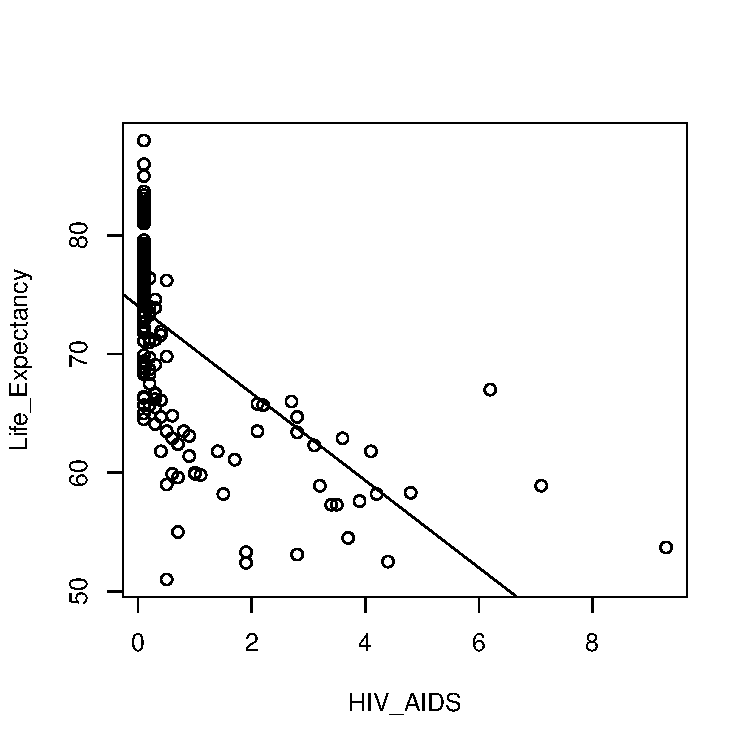
\includegraphics[width=\textwidth]{ProjectHIVPre.pdf}
		\end{subfigure}
		\begin{subfigure}[b]{0.49\textwidth}
			\centering
			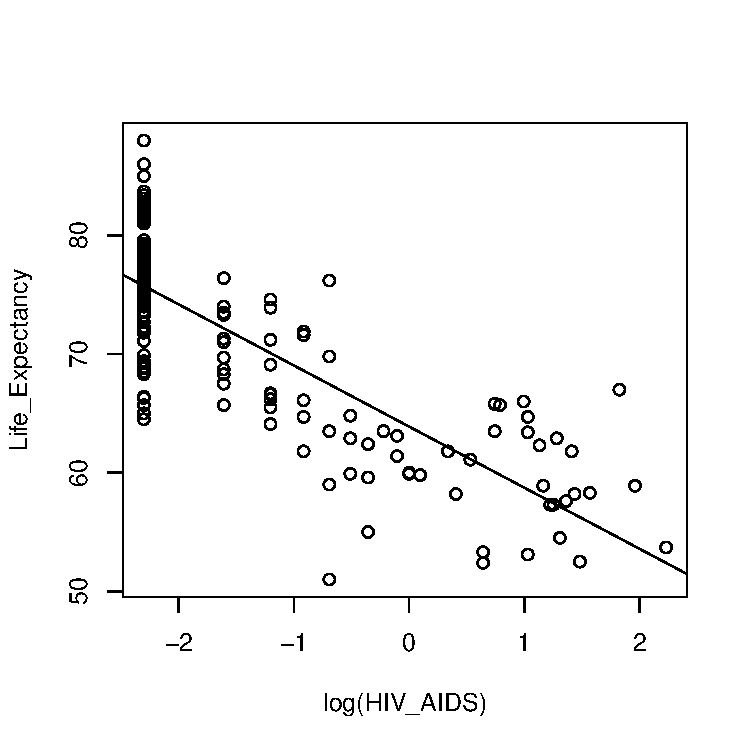
\includegraphics[width=\textwidth]{ProjectHIVPost.pdf}
		\end{subfigure}
		\begin{subfigure}[b]{0.49\textwidth}
			\centering
			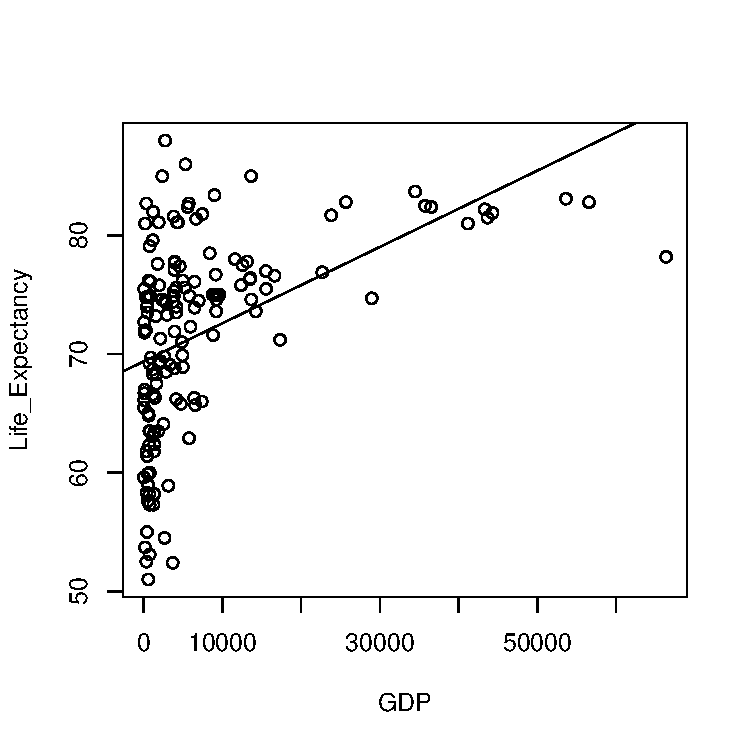
\includegraphics[width=\textwidth]{ProjectGDPPre.pdf}
		\end{subfigure}
		\begin{subfigure}[b]{0.49\textwidth}
			\centering
			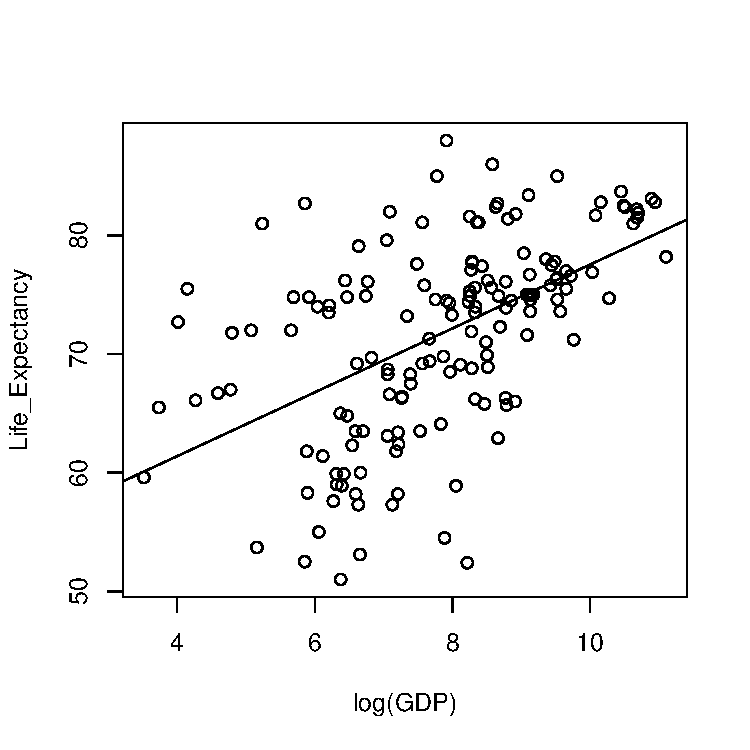
\includegraphics[width=\textwidth]{ProjectGDPPost.pdf}
		\end{subfigure}
	\caption{Before and after plots for the transformations performed on the HIV and GDP data sets.}
	\vspace{-3cm}
	\end{figure}
\newpage
	\begin{figure}[ht]
	\centering
		\begin{subfigure}[b]{0.49\textwidth}
			\centering
			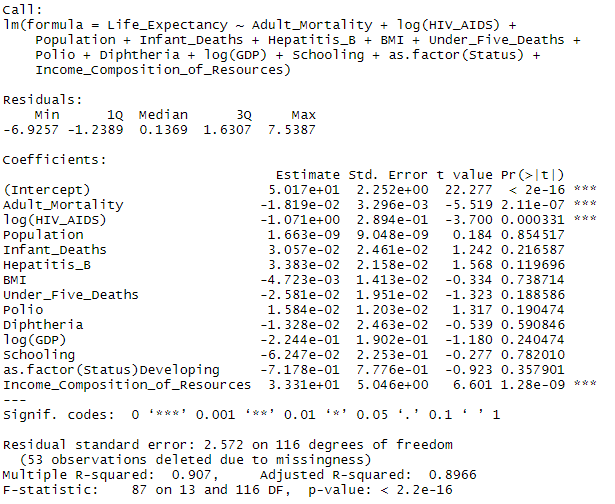
\includegraphics[width=\textwidth]{FullModelRegressionSummary.png}
		\end{subfigure}
		\begin{subfigure}[b]{0.49\textwidth}
			\centering
			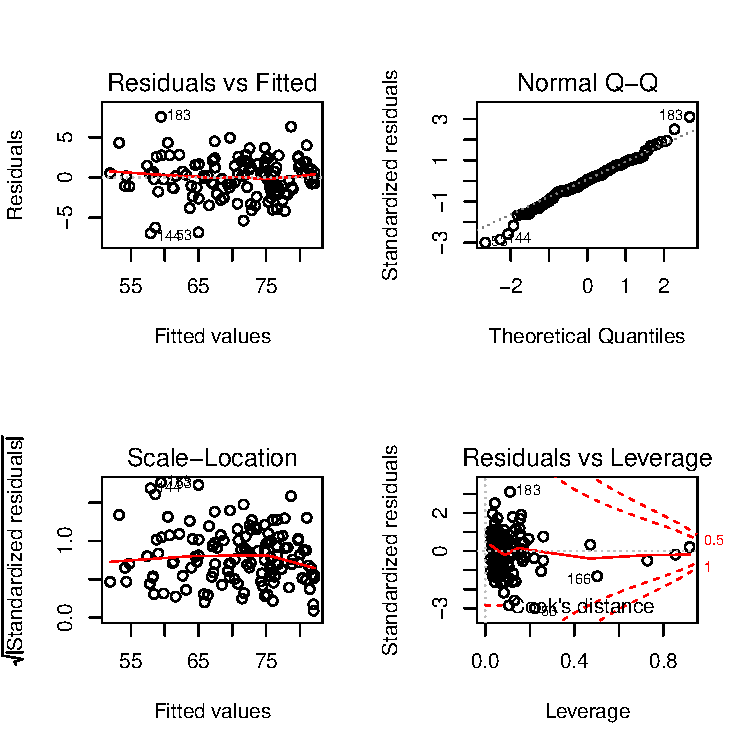
\includegraphics[width=\textwidth]{FullModelRegressionDiagnostics.pdf}
		\end{subfigure}
		\begin{subfigure}[b]{0.49\textwidth}
			\centering
			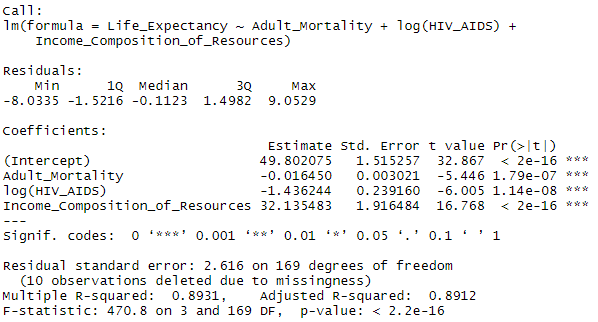
\includegraphics[width=\textwidth]{ResultModelRegressionSummary.png}
		\end{subfigure}
		\begin{subfigure}[b]{0.49\textwidth}
			\centering
			\includegraphics[width=\textwidth]{ResultModelRegressionDiagnostics.pdf}
		\end{subfigure}
	\caption{Before and after plots for the regression with all of the variables considered and with only the significant variables considered.}
	\vspace{-3cm}
	\end{figure}
\newpage
	\begin{figure}[ht]
	\centering
		\begin{subfigure}[b]{0.49\textwidth}
			\centering
			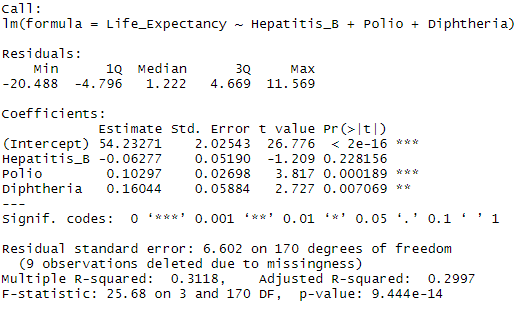
\includegraphics[width=\textwidth]{DiseaseModelRegressionSummary.png}
		\end{subfigure}
		\begin{subfigure}[b]{0.49\textwidth}
			\centering
			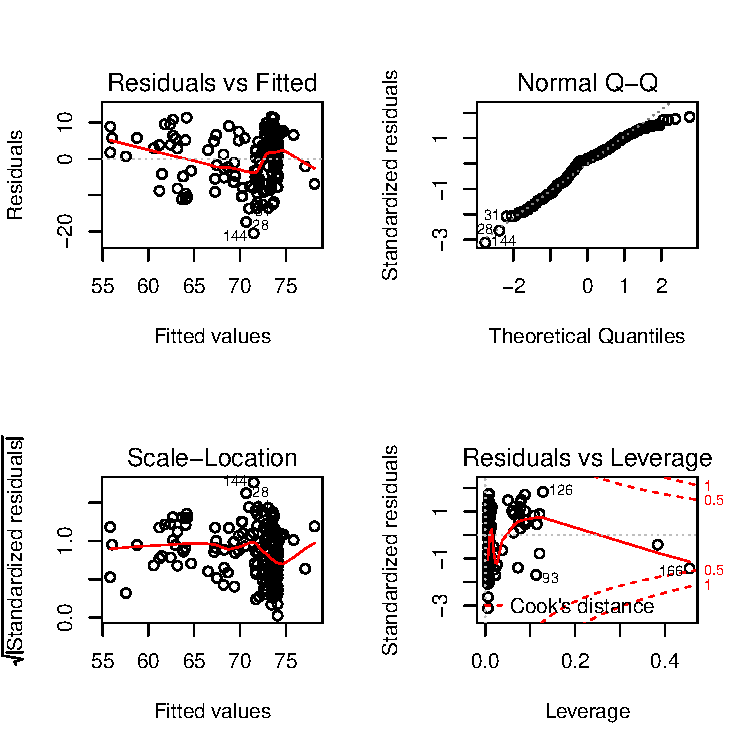
\includegraphics[width=\textwidth]{DiseaseModelRegressionDiagnostics.pdf}
		\end{subfigure}
	\caption{Regression summary and Diagnostic plots for the disease immunization tests.}
	\end{figure}

The data for this analysis was obtained from https://www.kaggle.com/kumarajarshi/life-expectancy-who
\end{document}